\documentclass[final,5p,times,twocolumn]{elsarticle}

\usepackage{lineno,hyperref}
\usepackage{times}
\usepackage{epsfig}
\usepackage{graphicx}
\usepackage{amsmath}
\usepackage{amssymb}
\usepackage{xcolor}
\modulolinenumbers[5]

\journal{Journal of \LaTeX\ Templates}

\bibliographystyle{elsarticle-num}
%%%%%%%%%%%%%%%%%%%%%%%

\begin{document}

\begin{frontmatter}

\title{Solução Numérica da Condução de Calor 2D}

%% Group authors per affiliation:
\author{José Henrique Zeferino - {\tt\small 190125985@aluno.unb.br}\\
Gustavo Policena Vitena - {\tt\small 190125764@aluno.unb.br}\\
}
\address{Universidade de Brasília}


\address[mymainaddress]{Campus Universitário Darcy Ribeiro, Faculdade de Tecnologia - Asa Norte, Brasília - DF, 70910-900}

\begin{abstract}
    In this article, we will determine the temperature at each point of a two-dimensional plate over time.
\end{abstract}

\begin{keyword}
Condução de calor 2D \sep solução numérica \sep condução bidimensional
\end{keyword}

\end{frontmatter}

\linenumbers
%=====================================================================================%
\section{Introdução}
\label{sec:Introdução}

Neste artigo, iremos determinar a temperatura em cada ponto de uma placa bidimensional ao longo do tempo. Mas, primeiro, iremos abordar certas teorias, como o princípio da conservação de energia e o método das diferenças finitas, a fim de apresentar o problema e compreender sua solução. Vale ressaltar que existem mais dois métodos para a resolução de problemas de condução bidimensional: o método da separação de variáveis e o método gráfico. No entanto, neste artigo, nos concentraremos no método numérico (diferenças finitas), que pode ser aplicado em diversas situações.

\subsection{Primeira Lei da Termodinâmica}
\label{sec:1 Lei da termodinamica}

A primeira lei da termodinâmica, também conhecida como princípio da conservação de energia, afirma que a energia total de um sistema isolado permanece constante ao longo do tempo. Em outras palavras, a variação da energia interna de um sistema ($\Delta U$) é igual à diferença entre o calor adicionado ao sistema ($Q$) e o trabalho realizado pelo sistema ($W$):

\begin{equation*}
    \Delta U = Q - W
\end{equation*}

Se considerarmos um sistema, como uma placa de comprimento 0 a x, onde um lado dessa placa é aquecido, e considerarmos que $Q$ será a energia que entra ($E_{entra}$) e que $W$ será a energia que sai ($E_{sai}$), conseguimos deduzir as seguintes equações:

\begin{equation*}
    \Delta E = E_{entra} - E_{sai} = E(t + \Delta t) - E(t)
\end{equation*}
\begin{equation*}
    E_{entra} = \dot{Q}(x)\Delta t
\end{equation*}
\begin{equation*}
    E_{sai} = \dot{Q}(x + \Delta x)\Delta t
\end{equation*}

Fazendo algumas substituições e lembrando que $\Delta E = mc\Delta T$:

\begin{equation*}
    E(t + \Delta t) - E(t) = (\rho c)V[T(t + \Delta t) - T(t)]
\end{equation*}

Onde $\rho c$ é a capacidade térmica do material, e $V$ é o volume do bloco onde $V = (\Delta x)A$, então temos que:

\begin{equation*}
    (\rho c)A\Delta x[T(t + \Delta t) - T(t)] = [\dot{Q}(x) - \dot{Q}(x + \Delta x)]\Delta t
\end{equation*}

\begin{equation*}
    (\rho c)A(\frac{T(t + \Delta t) - T(t)}{\Delta t}) = -(\frac{\dot{Q}(x + \Delta x) - \dot{Q}(x)}{\Delta x})
\end{equation*}

Assim fazendo $\Delta x \rightarrow 0$ e $\Delta t \rightarrow 0$, temos que:

\begin{equation*}
    (\rho c)A\frac{\partial T}{\partial t} = -\frac{\partial \dot{Q}}{\partial x}
\end{equation*}

ou

Como é possível ver na equação acima, a variação da temperatura ao longo do tempo só ocorre se houver uma variação na taxa de transferência de calor no espaço. No entanto, ainda não finalizamos, pois temos duas incógnitas. Para resolver isso, utilizaremos a Lei de Fourier, que estabelece que $\dot{Q} = -kA\frac{\partial T}{\partial x}$. Substituindo a Lei de Fourier na equação acima, temos:

\begin{equation*}
    \rho c\frac{\partial T}{\partial t} = k\frac{\partial}{\partial x}(\frac{\partial T}{\partial x})
\end{equation*}

Perceba que, a área ($A$) é constante, por conta parede ser plana, portanto podemos tirar ela da derivada parcial. Além disso, vamos aproximar a condutividade térmica ($k$) como sendo uma constante, uma vez que, em muitos casos, essa consideração é válida, apesar de seu valor depender da temperatura. Desta forma, como $k$, $\rho$ e $c$ são constantes, conseguimos definir uma nova propriedade que se chamará de difusividade térmica ($\alpha$), onde $\alpha = \frac{k}{\rho c}$.
Dessa forma, realizando as substituições mencionadas, chegamos à equação da condução de calor ou equação da difusão de calor:

\begin{equation}
\label{eq:condução de calor unidimensional}
    \frac{\partial T}{\partial t} = \alpha \frac{\partial^2 T}{\partial x^2}
\end{equation}

Lembrando que o caso anterior era para uma situação unidimensional. No caso geral, não podemos considerar a condutividade térmica ($k$) como constante, uma vez que ela depende não apenas da temperatura, mas também da direção do fluxo de calor. Assim a equação geral da condução de calor pode ser expressa da seguinte forma:

\begin{equation}
\label{eq:condução de calor geral}
    \rho c\frac{\partial T}{\partial t} = \frac{\partial}{\partial x}(k_1\frac{\partial T}{\partial x}) +
                                          \frac{\partial}{\partial y}(k_2\frac{\partial T}{\partial y}) +
                                          \frac{\partial}{\partial z}(k_3\frac{\partial T}{\partial z})
\end{equation}
\subsection{Método das Diferenças Finitas}
\label{sec:Diferenças Finitas}

Este método envolve resolver equações diferenciais, dividindo seu domínio e aproximando-as pela série de Taylor:

\begin{equation}
\label{eq:Difenreça+}
    f(x+\Delta x) = f(x) + f'(x)\Delta x + \frac{f''(x)\Delta x^2}{2} + \frac{f'''(x)\Delta x^3}{6} + o(\Delta x^4)
\end{equation}

Assim temos que a derivada primeira pode ser escrita como:

\begin{equation*}
    f'(x) = \frac{f(x+\Delta x) - f(x)}{\Delta x} + o(\Delta x)
\end{equation*}

Que é conhecida como fórmula das diferenças progressivas. E também podemos obter a derivada de segunda ordem fazendo a seguinte suposição, como:

\begin{equation}
\label{eq:Difenreça-}
    f(x-\Delta x) = f(x) - f'(x)\Delta x + \frac{f''(x)\Delta x^2}{2} - \frac{f'''(x)\Delta x^3}{6} + o(\Delta x^4)
\end{equation}

Se somarmos a equação \ref{eq:Difenreça+} e \ref{eq:Difenreça-}:

\begin{equation*}
    f(x+\Delta x) + f(x-\Delta x) = 2f(x)+f''(x)\Delta x^2 + o(\Delta x^4)
\end{equation*}

Obtemos a equação da derivada de segunda ordem:

\begin{equation}
\label{eq:DiferençaSegundaOrdem}
    f''(x)=\frac{f(x+\Delta x) - 2f(x) + f(x-\Delta x)}{\Delta x^2} + o(\Delta x^2)
\end{equation}
%=====================================================================================%
\section{Desenvolvimento}

Para facilitar o entendimento, vamos primeiro mostrar o desenvolvimento para o caso unidimensional.

\subsection{Unidimensional}
\label{sec:Unidimensional}
Vamos começar considerando a equação \ref{eq:condução de calor unidimensional}. Para facilitar nossos cálculos posteriores, vamos considerar a difusividade térmica como 1 ($\alpha = 1 , \text{m}^2/\text{s}$). Utilizando o método das diferenças finitas, conforme mostrado na seção \ref{sec:Diferenças Finitas}, e fazendo algumas aproximações, como $T(x_i,t_k) \approx T_i^k$, $x_i = i\Delta x$, e $t_k = k\Delta t$, obtemos:

\begin{equation}
\label{eq:AproximaçãoTempo}
    \frac{\partial T}{\partial x}|_{x_i,t_k} \approx \frac{T_i^{k+1}-T_{i-1}^k}{\Delta x}
\end{equation}
\begin{equation}
\label{eq:AproximaçãoEspaço}
    \frac{\partial^2T}{\partial x^2}|_{x_i,t_k} \approx \frac{T_{i+1}^k - 2T_i^k + T_{i-1}^k}{\Delta x^2}
\end{equation}

Perceba que o termo $O(\Delta x^2)$, da equação \ref{eq:DiferençaSegundaOrdem}, foi desprezada em nossa equação final, pois ele resultaria em um valor muito próximo de zero. Portanto, é possível aproximar esse termo como zero.

Prosseguindo, dividimos o comprimento da barra em vários pedaços, onde cada segmento possui um comprimento $\Delta x = \frac{L}{N}$. Em seguida, definimos pontos de medição ao longo da barra, com um total de $N$ pontos, e a temperatura em cada ponto será denotada como $T_i$. Além disso, como a temperatura varia tanto no espaço quanto no tempo, consideraremos $\Delta t$ como o intervalo entre duas medições consecutivas e $k$ como o instante de tempo em que a temperatura está sendo medida. Vale lembrar que para que este método obtenha uma aproximação boa, é necessário o uso do critério de estabilidade para $\Delta t$, ou seja, como $T^0 > 0$ então $\Delta t < 0.2*\Delta x^2$, e utilizaremos esse critério para a resolução dos nossos problemas.

Desta forma, avançando com a equação diferencial original (\ref{eq:condução de calor unidimensional}), e fazendo as substituições com as equações \ref{eq:AproximaçãoTempo} e \ref{eq:AproximaçãoEspaço}, obtemos o seguinte resultado:

\begin{equation*}
    \frac{T_i^{k+1}-T_{i-1}^k}{\Delta x} = \frac{T_{i+1}^k - 2T_i^k + T_{i-1}^k}{\Delta x^2}
\end{equation*}

E resolvendo essa equação, isolando o termo $T_i^{k+1}$, obtemos:

\begin{equation}
    T_i^{k+1} = T_i^k + \frac{\Delta t}{\Delta x^2}(T_{i+1}^k - 2T_i^k + T_{i-1}^k)
\end{equation}

Efetuamos todas essas etapas para simplificar a equação e assim consegui implementar um programa em Python que fará uma serie de simulações com vários valores diferentes...

...

\textcolor{red}{JOSÉ COLOCA A PARTE DO CÓDIGO DA BARRA UNIDIMENSIONAL AQUI}

...

Note que, para a resolver essa equação, são necessárias condições de contorno. E assim vamos para os nossos três problemas distintos, nos quais será aquecido uma barra de comprimento L e mudaremos as condições de contorno em cada problema. Em seguida, compararemos os valores obtidos por meio da aproximação com a solução exata fornecida.

\subsubsection{Problema 1}
\label{subsec:Problema 1}

Neste problema temos uma barra de 1 metro de comprimento que será dividida em 1000 partes, $N = 1000$, e calcularemos ate um tempo de 2 segundos. As condições de contorno serão:

\begin{itemize}
    \item $T(0,t) = 0$
    \item $T(L,t) = 0\\$
    para $t\ge 0$
    \item $T(x,0) = 1\\$
    para $0 < x < L$
\end{itemize}

\subsubsection{Problema 2}
\label{subsec:Problema 2}

Neste problema temos uma barra de 1 metro de comprimento que será dividida em 1000 partes, $N = 1000$, e calcularemos ate um tempo de 2 segundos. As condições de contorno serão:

\begin{itemize}
    \item $T(0,t) = 1$
    \item $T(L,t) = 0\\$
    para $t\ge 0$
    \item $T(x,0) = 0\\$
    para $0 < x < L$
\end{itemize}

\subsubsection{Problema 3}
\label{subsec:Problema 3}

Neste problema temos uma barra de 2 metro de comprimento que será dividida em 1000 partes, $N = 1000$, e calcularemos ate um tempo de 2 segundos. As condições de contorno serão:

\begin{itemize}
    \item $T(0,t) = 0$
    \item $T(L,t) = 0\\$
    para $t\ge 0$
    \item $T(x,0) = sin(\frac{\pi * x}{2}\\$
    para $0 < x < L$
\end{itemize}

\subsection{Bidimensional}


Para resolver o nosso problema bidimensional, no qual uma placa quadrada é aquecida na superfície de superior e resfriado nas laterais e inferior, seguiremos um procedimento semelhante ao que fizemos na condução unidimensional. Primeiramente, precisamos resolver o problema da equação \ref{eq:condução de calor unidimensional}, onde a condutividades térmicas não serão constantes, uma vez que depende da direção. Para simplificar o problema, faremos uma aproximação considerando $k_1$ e $k_2$ como constantes iguais, uma vez que estamos trabalhando com eixos de mesmo comprimento devido à placa ser quadrada. Com essa simplificação, podemos expressar a equação geral de forma mais simples:

\begin{equation*}
    \frac{\partial T}{\partial t} = \alpha(\frac{\partial^2T}{\partial x^2} +
                                          \frac{\partial^2T}{\partial y^2})
\end{equation*}

Onde $\alpha = \frac{k}{\rho c}$, e novamente para facilitar as contas consideraremos $\alpha = 1 m^2/s$. Desta forma, a dedução feita na equação \ref{eq:AproximaçãoEspaço}, usada para $x$, também será usada para $y$. No entanto, agora teremos não apenas a temperatura no ponto $i$ ($T_i$), mas também a temperatura no ponto j ($T_j$). Desta maneira, a temperatura dependerá de ambos os pontos, resultando em:

\begin{itemize}
    \item $T(x_i, y_j, t_k) \approx T_{i,j}^k$
    \item $x_i = i\Delta x$
    \item $y_j = j\Delta y$
    \item $t_k = k\Delta t$
\end{itemize}

Agora utilizando as equações acimas nas deduções que já fizemos, obtemos:

\begin{equation}
    T_{i,j}^{k+1} = T_{i,j}^k + \frac{\Delta t}{\Delta x^2}(T_{i+1,j}^k - 2T_{i,j}^k + T_{i-1,j}^k)
                              + \frac{\Delta t}{\Delta y^2}(T_{i,j+1}^k - 2T_{i,j}^k + T_{i,j-1}^k) 
\end{equation}

Destarte, usando a equação acima conseguimos e as condições de contorno que já foi dado, conseguimos implementar um código em Python para fazer simulações...

...

\textcolor{red}{JOSÉ COLOCA A PARTE DO CÓDIGO DA PLACA BIDIMENSIONAL AQUI}

...




%=====================================================================================%
\section{Resultados}

\subsection{Resultado Problema 1}
\label{sec:ResultadoP1}

\begin{figure}[h]
    \centering
    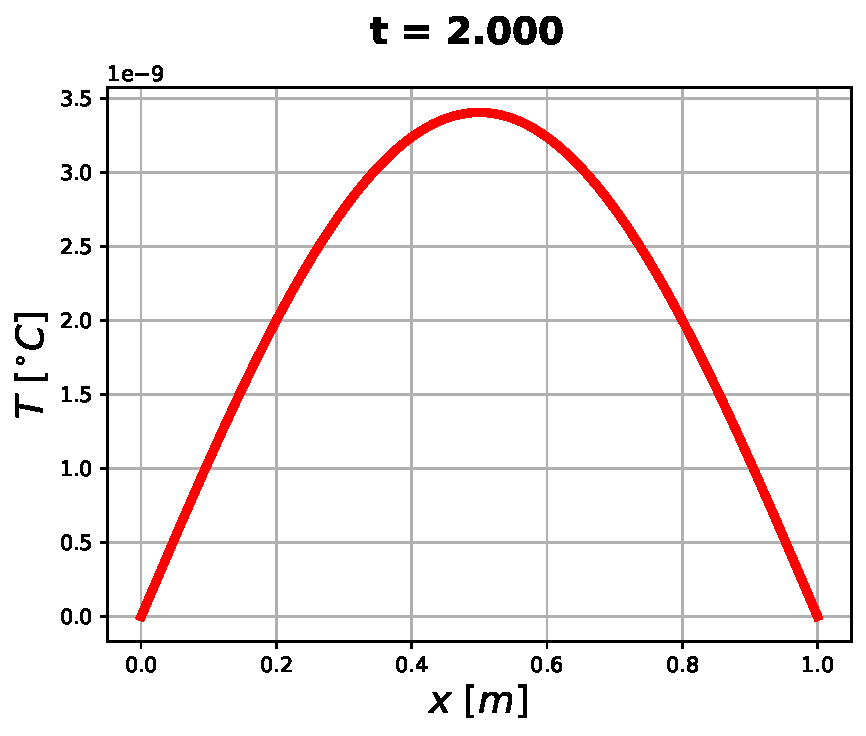
\includegraphics[width=0.4\textwidth]{Imagens/P1_T2s.pdf}
    \caption{Gráfico da Temperatura pela distancia em um período de 2 segundos}
    \label{fig:mesh1}
\end{figure}

Agora comparando com a solução exata, feita no programa MatLab:

\begin{figure}[h]
    \centering
    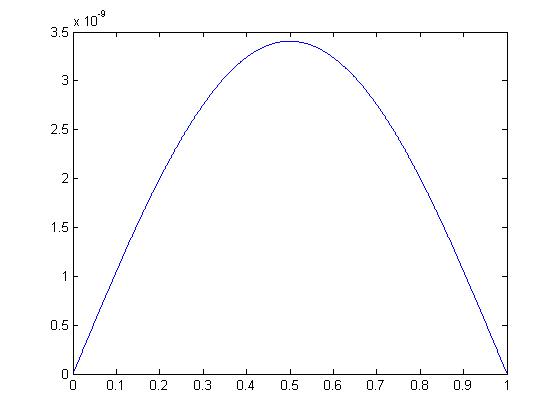
\includegraphics[width=0.4\textwidth]{Imagens/Matlab/P1_T2_MATHLAB.jpg}
    \caption{Gráfico da Temperatura pela distancia em um período de 2 segundos feito no matlab}
    \label{fig:mesh1}
\end{figure}

\subsection{Resultado Problema 2}
\label{sec:ResultadoP2}

\begin{figure}[h]
    \centering
    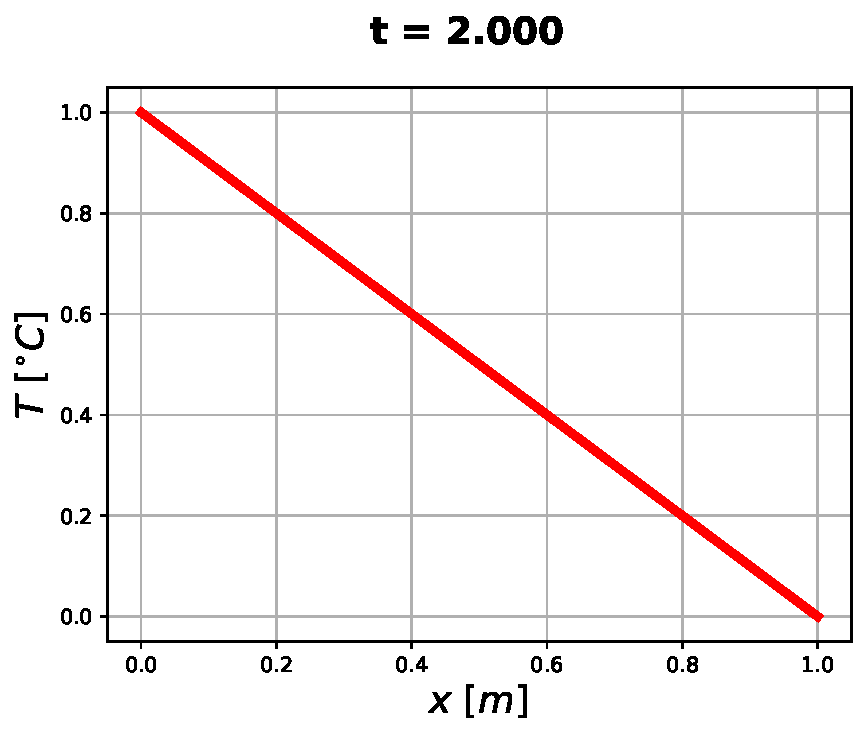
\includegraphics[width=0.4\textwidth]{Imagens/P2_T2.pdf}
    \caption{Gráfico da Temperatura pela distancia em um período de 2 segundos}
    \label{fig:mesh1}
\end{figure}

Agora comparando com a solução exata, feita no programa MatLab:

\begin{figure}[h]
    \centering
    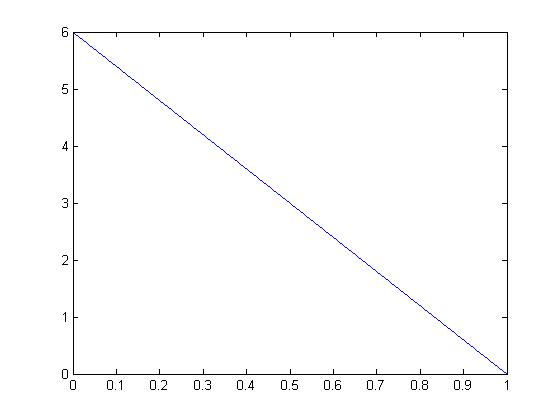
\includegraphics[width=0.4\textwidth]{Imagens/Matlab/P2_T2_MATHLAB.jpg}
    \caption{Gráfico da Temperatura pela distancia em um período de 2 segundos feito no matlab}
    \label{fig:mesh1}
\end{figure}

\subsection{Resultado Problema 3}
\label{sec:ResultadoP3}

\begin{figure}[h]
    \centering
    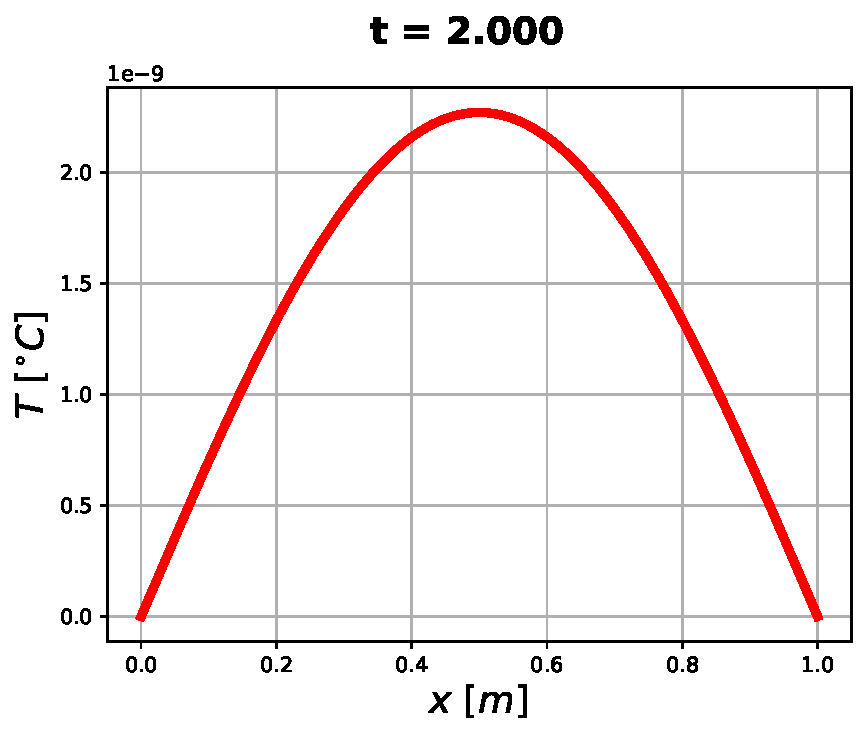
\includegraphics[width=0.4\textwidth]{Imagens/P3_T2.pdf}
    \caption{Gráfico da Temperatura pela distancia em um período de 2 segundos}
    \label{fig:mesh1}
\end{figure}

Agora comparando com a solução exata, feita no programa MatLab:

\begin{figure}[h]
    \centering
    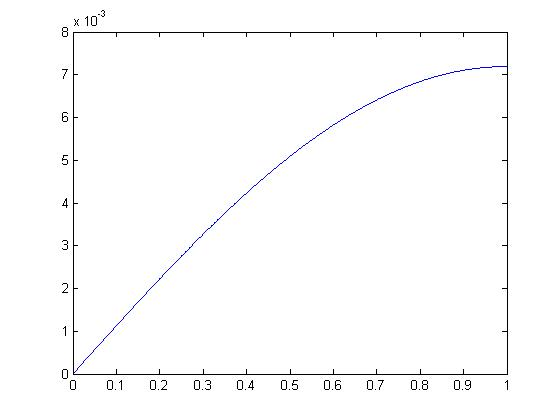
\includegraphics[width=0.4\textwidth]{Imagens/Matlab/P3_T2_MATHLAB.jpg}
    \caption{Gráfico da Temperatura pela distancia em um período de 2 segundos feito no matlab}
    \label{fig:mesh1}
\end{figure}

\subsection{Resultado Problema Bidimensional}

\begin{figure}[h]
    \centering
    
\includegraphics[width=0.4\textwidth]{Imagens/example.jpg}
    \caption{Gráfico da Temperatura pela distancia em x e y em um período de 2 segundos}
    \label{fig:mesh1}
\end{figure}

%=====================================================================================%
\section{Conclusão}

...\\
...\\
...\\




%=====================================================================================%
\section*{Referências}

\bibliography{mybibfile}

\end{document}
